\documentclass[
% -- opções da classe memoir --
12pt,				% tamanho da fonte
openright,			% capítulos começam em pág ímpar (insere página vazia caso
%preciso)
twoside,			% para impressão em recto e verso. Oposto a oneside
a4paper,			% tamanho do papel. 
% -- opções da classe abntex2 --
%chapter=TITLE,		% títulos de capítulos convertidos em letras maiúsculas
%section=TITLE,		% títulos de seções convertidos em letras maiúsculas
%subsection=TITLE,	% títulos de subseções convertidos em letras maiúsculas
%subsubsection=TITLE,% títulos de subsubseções convertidos em letras maiúsculas
% -- opções do pacote babel --
english,			% idioma adicional para hifenização
french,				% idioma adicional para hifenização
spanish,			% idioma adicional para hifenização
brazil				% o último idioma é o principal do documento
]{abntex2_new}

% ---
% Pacotes básicos 
% ---
\usepackage{lmodern}			% Usa a fonte Latin Modern			
\usepackage[T1]{fontenc}		% Selecao de codigos de fonte.
\usepackage[utf8]{inputenc}		% Codificacao do documento (conversão automática
%dos acentos)
\usepackage{lastpage}			% Usado pela Ficha catalográfica
\usepackage{indentfirst}		% Indenta o primeiro parágrafo de cada seção.
\usepackage{color}				% Controle das cores
\usepackage{graphicx}			% Inclusão de gráficos
\usepackage{microtype} 			% para melhorias de justificação
\usepackage{amsmath}

% ---

% ---
% Pacotes adicionais, usados apenas no âmbito do Modelo Canônico do abnteX2
% ---
\usepackage{lipsum}				% para geração de dummy text
% ---

% ---
% Pacotes de citações
% ---
\usepackage[brazilian,hyperpageref]{backref}	 % Paginas com as citações na bibl
\usepackage[alf]{abntex2cite}	% Citações padrão ABNT
\usepackage{listings}


\definecolor{codegreen}{rgb}{0,0.6,0}
\definecolor{codegray}{rgb}{0.5,0.5,0.5}
\definecolor{codepurple}{rgb}{0.58,0,0.82}
\definecolor{backcolour}{rgb}{0.95,0.95,0.92}

\lstdefinestyle{mystyle}{
	backgroundcolor=\color{backcolour},   
	commentstyle=\color{codegreen},
	keywordstyle=\color{magenta},
	numberstyle=\tiny\color{codegray},
	stringstyle=\color{codepurple},
	basicstyle=\footnotesize,
	breakatwhitespace=false,         
	breaklines=true,                 
	captionpos=b,                    
	keepspaces=true,                 
	numbers=left,                    
	numbersep=5pt,                  
	showspaces=false,                
	showstringspaces=false,
	showtabs=false,                  
	tabsize=2
}

\lstset{style=mystyle}
\lstset{language=Python}
% --- 
% CONFIGURAÇÕES DE PACOTES
% --- 

% ---
% Configurações do pacote backref
% Usado sem a opção hyperpageref de backref
\renewcommand{\backrefpagesname}{Citado na(s) página(s):~}
% Texto padrão antes do número das páginas
\renewcommand{\backref}{}
% Define os textos da citação
\renewcommand*{\backrefalt}[4]{
	\ifcase #1 %
	Nenhuma citação no texto.%
	\or
	Citado na página #2.%
	\else
	Citado #1 vezes nas páginas #2.%
	\fi}%
% ---

% ---
% Informações de dados para CAPA e FOLHA DE ROSTO
% ---
\titulo{Trabalho de Modelagem Computacional}
\autor{Pedro Pacheco Mendes Filho}
\local{Santarém, Pará}
\data{2018}
\orientador{Dra. Marciana Lima Góes}
\instituicao{%
	Universidade Federal do Oeste do Pará
	\par
	Instituto de Engenharia e Geociência
	\par
	Programa de Ciência e Tecnologia}
\tipotrabalho{Trabalho Acadêmico}
% O preambulo deve conter o tipo do trabalho, o objetivo, 
% o nome da instituição e a área de concentração 
\preambulo{Esse trabalho foi criado como avaliador na obtenção de nota para
	a disciplina de Modelagem Computacional.}
% ---


% ---
% Configurações de aparência do PDF final

% alterando o aspecto da cor azul
\definecolor{blue}{RGB}{41,5,195}

% informações do PDF
\makeatletter
\hypersetup{
	%pagebackref=true,
	pdftitle={\@title}, 
	pdfauthor={\@author},
	pdfsubject={\imprimirpreambulo},
	pdfcreator={LaTeX with abnTeX2},
	pdfkeywords={abnt}{latex}{abntex}{abntex2}{trabalho acadêmico}, 
	colorlinks=true,       		% false: boxed links; true: colored links
	linkcolor=blue,          	% color of internal links
	citecolor=blue,        		% color of links to bibliography
	filecolor=magenta,      		% color of file links
	urlcolor=blue,
	bookmarksdepth=4
}
\makeatother
% --- 

% --- 
% Espaçamentos entre linhas e parágrafos 
% --- 


\setlength{\parindent}{1.3cm}


\setlength{\parskip}{0.2cm}  


\makeindex
% ---


\begin{document}
	
	
	\selectlanguage{brazil}
	
	\frenchspacing 
	
	
	\imprimircapa
	
	
	\imprimirfolhaderosto*
	
	
	\begin{fichacatalografica}
		\sffamily
		\vspace*{\fill}					% Posição vertical
		\begin{center}					% Minipage Centralizado
			\fbox{\begin{minipage}[c][8cm]{13.5cm}		% Largura
					\small
					\imprimirautor
					
					
					\hspace{0.5cm} \imprimirtitulo  / \imprimirautor. --
					\imprimirlocal, \imprimirdata.
					
					\hspace{0.5cm} \pageref{LastPage} p.\\
					
					\hspace{0.5cm} \imprimirorientadorRotulo~\imprimirorientador\\
					
					\hspace{0.5cm}
					\parbox[t]{\textwidth}{\imprimirtipotrabalho~--~\imprimirinstituicao,
						\imprimirdata.}\\
					
					
				\end{minipage}}
			\end{center}
		\end{fichacatalografica}
		
		
		\clearpage
		
		\setlength{\absparsep}{18pt}
		\begin{resumo}
			Esse trabalho tem como objetivo demonstrar o uso de métodos iterativos,
			no caso, de Gauss-Jacobi e Gauss-Seidel, para a resolução de sistemas lineares
			propostos e relacionando a problemas comuns, para fins de demonstrar suas 
			diferenças enquanto desempenho e precisão. Além disso, mostrar como a
			Modelagem 
			Computacional é um ótimo recurso  para resolução de  problemas de cálculo 
			como operações matriciais, sistemas,
			somatória e equações lineares.
			
			\textbf{Palavras-chave}: Gauss-Jacobi. Gauss-Seidel. Métodos Iterativos.
			Sistemas Lineares. Modelagem Computacional.
		\end{resumo}
		
		\pdfbookmark[0]{\contentsname}{toc}
		\tableofcontents*
		
		
		\textual
		
		
		% ----------------------------------------------------------
		\chapter*[Introdução]{Introdução}
		\addcontentsline{toc}{chapter}{Introdução}
		% ----------------------------------------------------------
		A resolução de sistemas lineares é muito importante para a resolução de
		problemas
		reais, para isso usamos a solução numérica com auxílio computacional para
		resolver
		e solucionar problemas de maneira rápida e precisa. O sistema linear é descrito
		por 
		$m$ equações com $n$ incógnitas $x_i$ como em: $a_{i1} x_1 + a_{i2} x_2 + ... +
		a_{in} x_n = b_i$, 
		e é usualmente representado na forma matricial $Ax = b$, que facilita a
		visualização
		computacional.
		
		Os métodos iterativos usados para achar o valor aproximado, partindo de um valor
		inicial
		e calculando a discretização numérica se aproximando cada vez do resultado, até
		o erro ser inferior à
		tolerância, significando assim a convergência do método; ou quando o número de iterações
		exceder o limite definido, portanto, não convergindo a um resultado. Pode se achar
		 resultado
		tão aproximado quanto
		queira, mas a baixa tolerância pode significar um número de iterações muito
		grande e talvez desnecessário.
		
		O método de Gauss-Jacob e Gauss-Seidel usados na resolução dos problemas necessitam de alguns
		parâmetros, são eles, 
		o sistema, o chute inicial, a tolerância desejada e também o
		limite de iterações.
		
		Será apresentado o algoritmo desenvolvido em Python, tanto para teste de
		critérios de covergência: 
		critério de linha, diagonal dominante e critério de Sassenfeld; e também a
		resolução do método de 
		Gauss-Jacob.
		
		Os resultados serão demonstrados pelo método de Gauss-Jacob, será apresentado
		algumas iterações,
		o gráfico de rapidez de covergência e os parâmetros usados na resolução.
		
		% ----------------------------------------------------------
		\chapter{Método de Gauss-Jacob}
		% ----------------------------------------------------------
		
		O método de Gauss-Jacobi permite obter-se uma solução única para um sistema
		$Ax=b, A = (a_{ij} ) $ com 
		$i,j=1,...,n$ e $det(A) \neq 0$. É denominado iterativo porque fornece uma
		sequência de raízes aproximadas
		obtidas através dos resultados anteriores. A construção do método é descrito
		como a transformação do 
		sistema $Ax = b$ para forma $x = Cx + d$ , que a partir dela, lança-se um valor
		inicial para o sistema, 
		para encontrar a primeira solução aproximada, dando início ao processo iterativo
		do método, porém 
		só será executado se os critérios de convergência forem atendidos.
		
		\section{Valores Iniciais}
		Primeiramente, para a execução de um sistema pelo método, é 
		necessário definir os valores iniciais para aquele 
		específico problema. São parâmetros como as funções do
		sistema,
		chute inicial, tolerância, limite de iterações e número
		de variáveis.
		
		Esses parâmetros tem como características:
		
		\begin{alineas}
			\item{\textbf{Funções do sistema:}\\
				As funções são colocadas em forma de matriz para que
				analise e resolva de forma rápida através de operações
				matriciais:
				
				$$\left.\begin{aligned}
				A=a_{1A} x + a_{2A} y\\
				B=a_{1B} x + a_{2B} y
				\end{aligned}
				\right\} \rightarrow
				\begin{bmatrix}
				a_{1A} & a_{2A} \\
				a_{1B} & a_{2B}
				\end{bmatrix} \cdot
				\begin{bmatrix}
				x \\
				y
				\end{bmatrix}
				= 
				\begin{bmatrix}
				A \\
				B
				\end{bmatrix}
				$$\\
				$$Ax=b$$
				
				No algoritmo, elas são definidas e armazenadas em variáveis como:
				$$	A \rightarrow   \begin{bmatrix}
				a_{1A} & a_{2A} \\
				a_{1B} & a_{2B}
				\end{bmatrix} \hspace{25pt}
				b \rightarrow  \begin{bmatrix}
				A \\
				B
				\end{bmatrix}
				$$\\
				
				Em exemplo, ele se apresenta dessa forma:
				
				$$	A \rightarrow   \begin{bmatrix}
				1 & 2 & 3 \\
				2 & 5 & 6 \\
				2 & 3 & 4
				\end{bmatrix} \hspace{25pt}
				b \rightarrow  \begin{bmatrix}
				23,5 \\
				50 \\
				36
				\end{bmatrix}
				$$\\
				
				Agora no Python,\\
				
				
				\begin{lstlisting}
				A = numpy.array([[1,2,3],
				[2,5,6],
				[2,3,4]], dtype=float)
				
				b = [23.5,50,36]
				\end{lstlisting}
				A bibilioteca \textit{numpy} servirá para auxiliar nas operações matriciais.
			}
			
			\item{\textbf{Chute Inicial}\\
				Em valores iniciais você define os valores $b$ para cada
				equação do sistema. No caso, esses valores vem de analise previamente feitas do
				sistema. O chute inicial
				vai ser determinante para definir a quantidade de 
				iterações necessárias para que se encontre o valor
				aproximado, de acordo com a tolerância definida, de 
				cada raiz.
				
				$$  \begin{bmatrix}
				x \\
				y \\
				z 
				\end{bmatrix} =
				\begin{bmatrix}
				0 \\
				0 \\
				0
				\end{bmatrix}
				$$\\
				
				E no Python,
				
				\begin{lstlisting}
				chute_inicial = [0,0,0]\end{lstlisting}
				
				
			}
			
			
			
			\item{\textbf{Tolerância:}\\
				A tolerância é o valor menor valor de aproximação da
				raiz aceito pelo algoritmo. Quanto menor o valor, maior
				será a precisão do método, porém, aumentará também o 
				número de iterações. Nos problemas, definimos como padrão
				a tolerância de $1\times10^{-3}$. No python, fica:
				\begin{lstlisting}
				tolerancia=  1E-3\end{lstlisting}
			}
			
			\item{\textbf{Limite de iterações:}\\
				O limite de iterações é necessário para o caso de houver
				erros programas e levar ao programa executar inúmeras iterações
				e entrando em um \textit{loop infinito}, fazendo o código executar cálculos
				desnecessário e ocupando muita memória. Definimos por padrão, o número limite
				de iterações como $1\times 10^{3}$. No Python, fica:
				\begin{lstlisting}
				iterMax=  1E3\end{lstlisting}
				
			}
			
			\item{\textbf{Números de Variáveis:}\\
				No caso do número de variáveis é necessário para alguns cálculos. No caso,
				fazemos 
				com que Python detecte de forma automática o tamanho da primeira linha da matriz
				$A$, 
				e defina como número de coeficientes, logo, também o número de variáveis. No
				algoritmo, fica:
				\begin{lstlisting}
				coef = A[0,:].size\end{lstlisting}
			}
			
			\item{\textbf{Tratamento da Matriz:}\\
				
				
			}
			
		\end{alineas}
		
		
		
		
		\section{Critérios de Convergência}
		Os critérios de convergência que envolve o método iterativo de Gauss-Jacobi, são
		esses:
		
		
		\begin{alineas}
			\item{\textbf{Critério de Linha:}
				$$\substack{\max \\ 1 \leq i \leq n} = \sum_{\substack{i = 1 \\ j \neq i}}^{n}
				|a_{ij}^{*} | < 1 $$
				Em Python,
				\begin{lstlisting}
				max_somatoria = 0
				for i in range(A[:,0].size):
				somatoria = 0
				for j in range(n):
				somatoria += abs(A[i,j])
				
				if(somatoria > max_somatoria):
				max_somatoria = somatoria
				
				if(max_somatoria < 2): 
				print("Criterio de Linha foi Atendido!")
				return True\end{lstlisting}
			}
			
			\item{\textbf{Se a matriz for diagonal dominante.}
				
				Em Python,
				\begin{lstlisting}
				diagonais = 0
				for i in range(A[:,0].size):
				if(A[i,i] > A[:,i].sum()-A[i,i] and A[i,i] > A[i,:].sum()-A[i,i]):
				diagonais +=1
				
				if diagonais == n:
				print('Criterio da Diagonal Dominante Atendido!')
				return True
				\end{lstlisting}
				
				
				
			}
			\item{\textbf{Critério de Sassenfeld:}
				$$\substack{\max \\ 1 \leq i \leq n}  \beta_i < 1 $$\hspace{25pt}, onde
				$$\beta_i = \sum_{j=1}^{i-1} |a_{ij}^{*} | \beta_j + \sum_{j = i + 1}^{n}  |
				a_{ij}^{*}|$$\\
				
				Em Python,
				\begin{lstlisting}
				max_sassenfeld = 0
				bj = [0]
				for i in range(A[:,0].size):
				bi = 0
				if i > 0:
				for j in range(A[:,0].size - 1):
				bi += abs(A[i,j]) * bj[j]
				
				for j in range(i + 1, n):
				bi += abs(A[i,j])
				
				bj.append(bi)
				
				if(bi >  max_sassenfeld):
				max_sassenfeld = bi
				
				if(max_sassenfeld < 1):
				print('Criterio de Sassenfeld foi Atentido!')
				return True\end{lstlisting}  
			}
		\end{alineas}
		
		No algoritmo, para executar os critérios do sistema, apresenta 
		primeiramente um tratamento, que é a divisão de cada equação pela sua diagonal,
		para
		facilitar o algoritmo na verificação do critério e para fins de analise.
		Nos problemas , todos os critérios são testados respectivamente como condição
		para
		execução do método, se um desses critérios forem atendido o método é executado.
		Se nenhum deles retornar um valor verdadeiro, o algoritmo cessará pois não irá
		convergir.
		
		
		\section{Algoritmo de Gauss-Jacob}
		O método, de forma geral, consiste em dado $x_0$, aproximação inicial, 
		obter aproximações através da relação recursiva $x{(k+1)}=Cx^k + d$.\\
		Para $i = 1,2,...,n$, podemos reescrever o sistema na (2.2) seguinte forma:\\
		$$x_i = \frac{b_i - \substack{\sum^{n} \\j=1,j \neq i}a_{ij}x_j}{a_{ii}}, i =
		1,2,...,n.$$\\
		até que o critério de parada seja satisfeito. Definiremos agora, o critério de
		parada e o 
		algoritmo de Gauss-Jacob.
		
		\begin{alineas}
			\item{\textbf{Critério de Parada}
				Os critérios de parada são usados para fim de não manter o algoritmo rodando
				quando o 
				resultado já é o bastante preciso e quando, por algum motivo, não alcançar a
				convergência.
				Há dois critérios que encerrara a execução do método, são eles:
				\subitem{\textbf{Máxima Iterações:}\\
					Será quando o limite de iterações forem atingidas, que poderá ser o caso de
					não convergência(serve para não sobrecarregar o computador quando não houver
					convergência).
				}
				\subitem{\textbf{Critério de distância:}\\
					Critério de distância avalia a precisão que o algoritmo chegou a partir do
					módulo da diferença da iteração atual e da anterior se o valor, porém o erro de
					cada variável do sistema tem que estar abaixo da tolerância para
					ser satisfeito:
					$$d^{(k)} = \substack{\max\\1 \leq i \leq n} |x_{i}^{(k)} - x_{i}^{(k-1)}| <
					\varepsilon_1$$
				}
				
				Então a condicional para execução do \textit{loop iterativo} do método, se torna
				em Python:
				
				
				\begin{lstlisting}
				iterAtual = 0 #Zerando as Iteracoes
				erro = 2      #Erro Inicial
				while(k < iterMax and erro >= tol):
				###Execucao do metodo
				\end{lstlisting}
				
				Enquanto, que o condicional presente dentro de \textit{while} resultar
				verdadeiro(\textit{True}), o método iterativo irá executar.
				
				\textit{Obs: A variável 'erro' é definido 2 apenas para fim que o condicional da
					iteração inicial resulte em verdadeiro, se não fosse definido, o método nunca
					iria executar.}
				
				
				
				
			}
			
			\item{\textbf{Algoritmo de Gauss Jacobi:}\\
				Agora, com todas as variáveis definidas, definiremos o método iterativo usado.
				Todos os
				valores entram no algoritmo do método e são executadas até que ache os valores
				das raízes, ou seja, a convergência.
				O algoritmo é auto-regulável, então, executará sistemas bidimensionais de
				tamanhos totalmente distintos.
				Seu desenvolvimento foi feito em Python, como apresentado logo abaixo:\\
				\begin{lstlisting}
				while(k < iterMax and erro >= tol):
				erro = 0		#Redefine o erro para iteracao atual
				
				xant = x.copy() #Copia os valores de 'x' antigos
				
				for i in range(n):
				soma = 0	#Redefine a somatoria para Iteracao atual
				for j in range(n):
				if(j != i):
				soma = soma + float(A[i,j])*xant[j]  #Metodo de Gauss-Jabob
				x[i] = (b[i] - soma)/float(A[i,i])		#Metodo de Gauss Jacob(se j = i)
				if(abs(x[i]-xant[i])>erro):	#Acha o Maximo erro das raizes
				erro = abs(x[i] - xant[i])
				k +=1 #Incremento da Iteracao
				\end{lstlisting}
				
			}	
		\end{alineas}
		
		\section{Algoritmo Completo}
		Apresentado abaixo o algoritmo completo om todas as definições e algumas f
		erramentas para analise como o \textit{matplotlib}(para plotagem de gráfico).
		
		\lstinputlisting{gauss.py}
		% ----------------------------------------------------------
		\chapter{Resolução de Problemas}
		Resolveremos problemas do cotiano para testar a veracidade do método, desempenho
		e
		precisão. Os parâmetros de entrada do problema serão:\\
		$$\left.\begin{aligned}
		A=a_{1A} x + a_{2A} y\\
		B=a_{1B} x + a_{2B} y
		\end{aligned}
		\right\} \rightarrow
		\begin{bmatrix}
		a_{1A} & a_{2A} \\
		a_{1B} & a_{2B}
		\end{bmatrix} \cdot
		\begin{bmatrix}
		x \\
		y
		\end{bmatrix}
		= 
		\begin{bmatrix}
		A \\
		B
		\end{bmatrix}
		$$\\
		$$	A \rightarrow   \begin{bmatrix}
		a_{1A} & a_{2A} \\
		a_{1B} & a_{2B}
		\end{bmatrix} \hspace{25pt}
		b \rightarrow  \begin{bmatrix}
		A \\
		B
		\end{bmatrix}
		$$\\
		
		\begin{alineas}
			\item{\textbf{Matriz de $A$}:\\
				A matriz dos coeficientes das variáveis:
				$$A \rightarrow   \begin{bmatrix}
				a_{1A} & a_{2A} \\
				a_{1B} & a_{2B}
				\end{bmatrix}$$}
			\item{\textbf{Matriz de $b$:}
				$$b \rightarrow  \begin{bmatrix}
				A \\
				B
				\end{bmatrix}$$
			}
			\item{\textbf{Chute Inicial: $x_1,x_2,x_3,...,x_n = 0$}\\
				
			}
			\item{\textbf{Tolerância:$1 \times 10^{-3}$}}
			\item{\textbf{Iterações Máxima:$1 \times 10^{3}$}}
		\end{alineas}
		
		E como resultado terá valores como:\\
		\begin{alineas}
			
			\item{\textbf{Critério de Convergência}:\\
				Em qual critério o sistema passou.}
			\item{\textbf{Número de Iterações:}\\
				Quantas iterações para achar o resultado com a tolerância desejada.}
			\item{\textbf{Primeiras Iterações:}\\
				O resultado das 3 primeiras iterações.}
			\item{\textbf{Resultado Obtido:}\\
				Resultado obtido pelo método com a tolerância desejada.
			}
			\item{\textbf{Gráfico de Convergência:}
				É o gráfico que demonstra qual a rapidez que o método convergiu para o
				resultado.
			}
		\end{alineas}
		
		
		\section{Transferência de calor em uma placa}
		Uma consideração importante no estudo da transferência de calor é a de
		se determinar a distribuição de temperatura assintótica de uma placa
		fina quando a temperatura em seu bordo é conhecida. Suponha que a placa
		represente uma seção transversal de uma barra de metal, com
		fluxo de calor desprezível na direção perpendicular à placa. Sejam
		$T_{1},..., T_6$ as temperaturas em seis vértices interiores do reticulado
		da figura. A temperatura num vértice é aproximadamente igual à média
		dos quatro vértices vizinhos mais próximos - à esquerda, acima, à direita,
		e abaixo. Por exemplo,\\
		
		$$T_1 = \frac{(10+20+T_2+T_4)}{4} \text{, ou } 4 T_1 - T_2 - T_4 = 30$$\\
		
		Escreva um sistema de seis equações cuja solução fornece estimativas para as
		temperaturas $T_1,...,T_6$.\\
		\begin{figure}[htb]
			\centering
			
			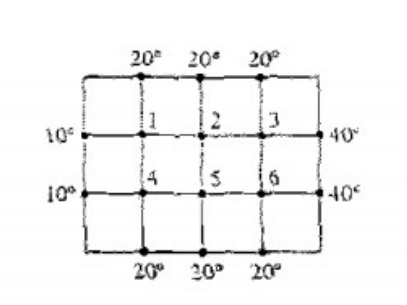
\includegraphics[scale=0.7]{figura1.png}
			
		\end{figure}
		
		Resolução:\\
		\\
		A solução desse problema primeiramente devemos encontrar o sistema. O próprio
		problema
		da um exemplo para seguir, então foi feito como demonstrado a definição do
		problema abaixo:\\
		$$\begin{cases}
		\begin{aligned}
		-4T_1+T_2+T_4=-30\\
		T_1-4T_2+T_3+T_5=-20\\
		T_2-4T_3+T_6=-60\\
		T-1-4T_4+T_5=-30\\
		T_2+T_4-4T_5+T_6=-20\\
		T_3+T_5-4T_6=-60
		\end{aligned}
		\end{cases}$$\\
		criando agora as matrizes $A$ e $b$:\\
		$$	A \rightarrow   \begin{bmatrix}
		-4 & 1 & 0 & 1 & 0 & 0 \\
		1 & -4 & 1 & 0 & 1 & 0 \\
		0 & 1 & -4 & 0 & 0 & 1 \\
		1 & 0 & 0 & -4 & 1 & 0 \\
		0 & 1 & 0 & 1 & -4 & 1 \\
		0 & 0 & 1 & 0 & 1 & -4 
		\end{bmatrix} \hspace{25pt}
		b \rightarrow  \begin{bmatrix}
		-30\\
		-20\\
		-60\\
		-30\\
		-20\\
		60
		\end{bmatrix}
		$$\\
		
		Colocando-a no algoritmo ela retornará os resultados:
		
		\begin{alineas}
			\item{\textbf{Critério de Convergência:} \textit{Critério de linha}.}
			\item{\textbf{Número de Iterações:}\textit{20}.}
			\item{\textbf{Precisão:}\textit{$7,14 \times 10^{-3}$}}
			\item{\textbf{Primeiras Iterações:}\\
				$$	\begin{bmatrix}
				0\\
				0\\
				0\\
				0\\
				0\\
				0
				\end{bmatrix} \rightarrow_1
				\begin{bmatrix}
				7,5\\
				5\\
				15\\
				7,5\\
				5\\
				15
				\end{bmatrix} \rightarrow_2
				\begin{bmatrix}
				10,625\\
				11,875\\
				20\\
				10,625\\
				11,875\\
				20
				\end{bmatrix} \rightarrow_3
				\begin{bmatrix}
				13,125\\
				15,625\\
				22,96875\\
				13,125\\
				15,625\\
				22,96875
				\end{bmatrix}$$
			}
			\item{\textbf{Resultado Obtido:}}\\
			$$\begin{bmatrix}
			17,142\\
			21,427\\
			27,142\\
			17,142\\
			21,427\\
			27,142
			\end{bmatrix}$$\\
			\clearpage
			\item{\textbf{Gráfico de Convergência:}}
			
			\begin{figure}[htb]
				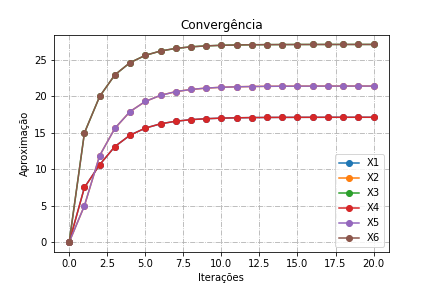
\includegraphics[scale=1]{grafico1.png}
				\legend{Gráfico de convergência de Gauss Jacob no sistema da placa transversal}
			\end{figure}
		\end{alineas}
		
		
		
		
		
		\section{Vitaminas equilibradas diariamente}
		Sabe-se que uma alimentação diária equilibrada em vitaminas deve constar
		de 170 unidades de vitamina A,
		180 unidades de vitamina C, 140 unidades
		de vitamina C, 180 unidades de vitamina D
		e 350 unidades de vitamina E.\\
		Com o objetivo de de descobrir como deverá
		ser uma refeição equilibrada, foram
		estudados cinco alimentos. Fixada na mesma quantidade (1g) de cada alimento
		, determinou-se:
		
		\begin{enumerate}
			\item{O alimento I tem 1 de unidade de vitamina A, 10 unidades de vitamina B, 1
				unidade de vitamina C, 2 unidades 
				de vitamina D e 2 unidades de vitamina E.}
			\item{O alimento II tem 9 unidades de vitamina A, 1 unidade de vitamina B, 0
				unidade de vitamina C, 1 unidade de 
				vitamina D e 1 unidade de vitamina E.}
			\item{O alimento III tem 2 unidades de A, 2 unidades de B, 5 unidades de C, 1
				unidade de D e 2 unidades de E.}
			\item{O alimento IV tem 1 unidade de A, 1 unidade de B, 1 unidade de C, 2
				unidades de D e 13 unidades de E.}
			\item{O alimento V tem 1 unidade de A, 1 unidade de B, 1 unidade de C, 9
				unidades de D e 2 unidades de E.}
		\end{enumerate}
		Quantos gramas de cada um dos alimentos I, II, III, IV e V devemos ingerir
		diariamente para que nossa alimentação seja
		equilibrada?\\
		\\Resolução:\\
		\\
		A solução desse problema primeiramente devemos encontrar o sistema. O sistema
		encontrado a partir da analise do problema foi esse:\\
		$$\begin{cases}
		\begin{aligned}
		1I+9II+2III+IV+V=170\\
		10I+II+2III+IV+V=180\\
		1I+0II+5III+IV+V=140\\
		2I+II+III+2IV+9V=180\\
		2I+II+2III+13IV+2V=350
		\end{aligned}
		\end{cases}$$\\
		criando agora as matrizes $A$ e $b$, já ajustadas, de modo de tentar a diagonal
		dominante, apenas trocando as posições da equações:\\
		$$	A \rightarrow   \begin{bmatrix}
		10 & 1 & 2 & 1 & 1  \\
		1 & 9 & 2 & 1 & 1  \\
		1 & 0 & 5 & 1 & 1  \\
		2 & 1 & 2 & 13 & 2  \\
		2 & 1 & 1 & 2 & 9  
		\end{bmatrix} \hspace{25pt}
		b \rightarrow  \begin{bmatrix}
		180\\
		170\\
		140\\
		350\\
		180
		\end{bmatrix}
		$$\\
		
		Colocando-a no algoritmo ela retornará os resultados:
		
		\begin{alineas}
			\item{\textbf{Critério de Convergência:} \textit{Critério de linha}.}
			\item{\textbf{Número de Iterações:}\textit{20}.}
			\item{\textbf{Precisão:}\textit{$6,05 \times 10^{-4}$}}
			\item{\textbf{Primeiras Iterações:}\\
				$$	\begin{bmatrix}
				0\\
				0\\
				0\\
				0\\
				0
				\end{bmatrix} \rightarrow_1
				\begin{bmatrix}
				18\\
				18,888\\
				28\\
				26,923\\
				20
				\end{bmatrix} \rightarrow_2
				\begin{bmatrix}
				5,818\\
				5,452\\
				15,015\\
				15,316\\
				4,807
				\end{bmatrix} \rightarrow_3
				\begin{bmatrix}
				12,439\\
				12,669\\
				22,811\\
				22,558\\
				13,029
				\end{bmatrix}$$
			}
			\item{\textbf{Resultado Obtido:}}\\
			$$\begin{bmatrix}
			9,9998\\
			9,9998\\
			19,9997\\
			19,9998\\
			9,9997
			\end{bmatrix}$$\\
			
			\item{\textbf{Gráfico de Convergência:}}
			
			\begin{figure}[htb]
				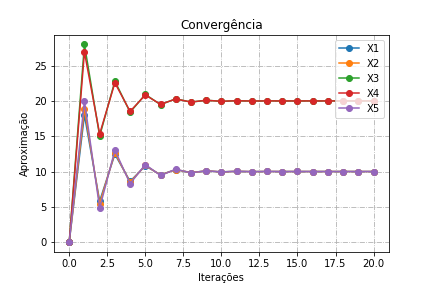
\includegraphics[scale=1]{grafico2.png}
				\legend{Gráfico de convergência de Gauss Jacob no sistema da vitaminas
					diárias}
			\end{figure}
		\end{alineas}
		
		\chapter{Conclusão}
		
		O método numérico de Gauss-Jacob é preciso e rápido para resolver sistemas,
		porém e limitado
		em questão de abrangência de sistema, pois, somente convergem sistemas se, e
		somente se, passar pelos seus \textit{Critérios de Convergência}. Por isso, não
		poderá ser usado
		para resolução para qualquer problema. A convergência de sistemas é rápida, por
		isso, é usual
		tratando sistemas grandes, pois pelo método convencional é inviável resolver
		número grande de equações
		e variáveis, ae que torna o método eficaz. Há também a possibilidade de
		paralelização de seu algoritmo, o que aumenta mais ainda a rapidez do código.
		
		
		% ----------------------------------------------------------
		%---------------------------------------------------------------------
		
	\end{document}
